\documentclass{article}
\usepackage[english]{babel}
\usepackage{enumerate, latexsym, amssymb, amsmath}
\usepackage{framed, multicol}
\usepackage{graphicx}
\usepackage{hyperref}
\newenvironment{forthel}{\begin{leftbar}}{\end{leftbar}}

%%%%%%%%%% Start TeXmacs macros
\newcommand{\tmaffiliation}[1]{\\ #1}
\newcommand{\tmem}[1]{{\em #1\/}}
\newenvironment{enumeratenumeric}{\begin{enumerate}[1.] }{\end{enumerate}}
\newenvironment{proof}{\noindent\textbf{Proof\ }}{\hspace*{\fill}$\Box$\medskip}
\newenvironment{quoteenv}{\begin{quote} }{\end{quote}}
\newenvironment{subproof}{\begin{list}{}{}
		\item[\text{Proof}]}{\hfill $\surd$ \end{list}}
\newenvironment{case}{\begin{list}{}{}
		\item[]}{\end{list}}	
\newtheorem{axiom}{Axiom}
\newtheorem{lemma}{Lemma}
\newtheorem{theorem}{Theorem}
\newtheorem{definition}{Definition}
\newtheorem{signature}{Signature}
\newtheorem{proposition}{Proposition}
%%%%%%%%%% End TeXmacs macros

\newcommand{\event}{UITP 2018}
\newcommand{\dom}{Dom}
\newcommand{\fun}{aFunction}
\newcommand{\sym}{sym}
\newcommand{\halfline}{{\vspace{3pt}}}
\newcommand{\tab}{{\hspace{1cm}}}
\newcommand{\ball}[2]{B_{#1}(#2)}
\newcommand{\llbracket}{[}
\newcommand{\rrbracket}{]}
\newcommand{\less}[1]{<_{#1}}
\newcommand{\greater}[1]{>_{#1}}
\newcommand{\leeq}[1]{{\leq}_{#1}}
\newcommand{\supr}[1]{\mathrm{sup}_{#1}}
\newcommand{\RR}{\mathbb{R}}
\newcommand{\QQ}{\mathbb{Q}}
\newcommand{\ZZ}{\mathbb{Z}}
\newcommand{\NN}{\mathbb{N}}
\newcommand{\cdotone}{\cdot}
\newcommand{\cdottwo}{\cdot}
\newcommand{\plusone}{+}
\newcommand{\plustwo}{+}
\newcommand{\halfeps}{\frac{\epsilon}{2}}
\newcommand{\inveps}{\frac{1}{\epsilon}}
\newcommand{\rooteps}{\sqrt{\epsilon}}
\newcommand{\dotequal}{=}


\begin{document}

\title{An SAD3 Formalization of Real Sequences for Walter Rudin's
\it{Principles of Mathematical Analysis}}

\author{Lukas Schembecker, Annika Hennes}

\date{September 10, 2018}

\maketitle


\section{Introduction}
The present formalization covers chapter 3 'Numerical Sequences (and Series)' (pages 47 to 58) of the {\it Principles of Mathematical Analysis} by Walter \linebreak Rudin \cite{Rudin}. We only focus on the part about Sequences and regard the special case of the metric space $\mathbb{R}$. We use the formalization of real numbers found in 'examples/Forster/Reals.ftl' and added a few more simple general real number facts, which the prover uses as auxiliary lemmata. To improve readability, we moved most of these to a seperate file - 'helper.ftl'.

\section{The Formalization}
\subsection{Sequences.ftl}

In order to improve the proof reading experience, we added two new enviroments 'subproof' and 'case' in LaTeX. These allow proofs being structured by further indentations. The parser needs to ignore these new enviroments, so we changed it's Haskell code in 'Alice/Import/LaTeX.hs' accordingly. Besides some further small changes, like changing the appearance of ' $+'$ ' to '$+$', we also tried to change the appearance of the absolute function 'abs' and the inverse function 'inv' to their standard representation, but to get them properly parsed one needs to do some more elaborate changes to the parser.\\

\noindent The definitions of sequences can be translated very closely to Rudin's text:

\begin{forthel}
	\noindent $\text{[read Sequences/Naturals.ftl]}\\
	\text{[read Sequences/helper.ftl]}\\
	\text{[sequence/-s]}
	\text{[converge/-s]}$\\
	Let $n$, $m$, $k$, $N$, $N1$, $N2$, $N3$ denote natural numbers.

	\begin{definition}
		$\NN$ is the set of natural numbers.
	\end{definition}
	
	\begin{definition}[Seq]	A sequence f is a function such that every element of Dom(f) is a natural number and every
	natural number is an element of $Dom(f)$ and for every $n \ f[n]$ is a real number.
	\end{definition}
	
	\begin{axiom}[SequenceEq] Let $a, b$ be sequences. \\ $a = b$ iff for every $n \ a[n] = b[n]$.
	\end{axiom}
	
	\begin{definition}[Convergence] Let $a$ be a sequence. Let $x$ be a real number. $a$ converges to $x$ iff for every positive real
	number $\epsilon$ there exists $N$ such that for every $n$ such that $N < n \ dist(a[n],x) < \epsilon$.
	\end{definition}
	
	\begin{definition}[Conv] Let $a$ be a sequence. $a$ converges iff there exists a real number $x$ such that $a$ converges to $x$.
	\end{definition}
	
	\noindent Let $a$ is convergent stand for $a$ converges.
	\\Let $a$ diverges stand for $\neg$ ($a$ converges).
	\\Let $a$ is divergent stand for $a$ diverges.
	
	\begin{definition}[Range] Let $a$ be a sequence. \\ $ran(a) = \{a[n] \mid \text{n is a natural number} \}$. 
	\end{definition}
\end{forthel}

\noindent Here we depart from the standard definition of finite range - namely the set theoretic finiteness of $ran$ - and use an equivalent definition, which is more related to the convergence definition as a set theoretic definition of finiteness is far more complex.

\begin{forthel}
	\begin{definition}[RangeN] Let $a$ be a sequence. \\ $ranN(a,N) = \{a[n] \mid \text{n is a natural number such that } n \leq N\}$. 
	\end{definition}
	
	\begin{definition}[FiniteRange]	Let $a$ be a sequence. $a$ has finite range iff there exists an $N$ such that $ran(a) = ranN(a,N)$.
	\end{definition}

	\begin{definition}[InfiniteRange] Let $a$ be a sequence. $a$ has infinite range iff $\neg$ ($a$ has finite range).
	\end{definition}
\end{forthel}

\noindent The following properties of $\frac{1}{n}$ and $(-1)^{n}$ are said to be trivial by Rudin as they only need 'common math' to be proven. A rigerous formalization needs to address these common facts seperately, so they text gets naturally longer.\\

\noindent Here we also have to consider the special case of $n=0$. Rudin does not consider 0 as a natural number.

\begin{forthel}
	\begin{lemma}[PropertiesOfInv]
		Let $a$ be a sequence such that for every $n$
		((If $n = 0$ then $a[n] = 2$) and (if $n \neq 0$ then $a[n] = inv(n)$)).
		Then $a$ converges to $0$ and $a$ has infinite range.
	\end{lemma}
	\begin{proof}
		Let us show that $a$ converges to $0$.
		\begin{subproof}
			Let $\epsilon$ be a positive real number. 
			Take $N$ such that $1 < N \cdot \epsilon$ \\(by ArchimedeanAxiom, OnePos).
	
			Let us show that for every $n$ such that $N < n \ dist(a[n],0) < \epsilon$.
			\begin{subproof}
				Assume $N < n$. Then $n \neq 0$.
				Let us show that $inv(n) < \epsilon$.
				\begin{subproof}
					We have $N \cdot \epsilon < n \cdot \epsilon$ (by ComMult, MultInvariance).\\
					Hence $1 < n \cdot \epsilon$ (by TransitivityOfOrder).\\
					$inv(n)$ is positive.\\
					Hence $inv(n) \cdot 1 < inv(n) \cdot (n \cdot \epsilon)$ (by MultInvariance).\\
					We have $inv(n) \cdot 1 = inv(n)$ (by One).
				
					$inv(n) \cdot (n \cdot \epsilon) \dotequal (inv(n) \cdot n) \cdot \epsilon$ (by AssMult)\\
					$\dotequal 1 \cdot \epsilon$ (by InvDummy)\\
					$\dotequal \epsilon$ (by OneDummy).
				\end{subproof}
				Hence $dist(a[n],0) = inv(n) < \epsilon$.
			\end{subproof}
		\end{subproof}
		Let us show that $a$ has infinite range.
		\begin{subproof}
			Assume the contrary.
			Take $N$ such that $ran(a) = ranN(a,N)$ \linebreak(by FiniteRange).
			Then $a[N + 1]$ is an element of $ran(a)$ (by OneNat, AddClosedNat, Range).
			
			Let us show that $a[N + 1]$ is not an element of $ranN(a,N)$.
			\begin{subproof}
				Let us show that for every natural number $n$ such that \\$n \leq N \ a[n] \neq a[N + 1]$.
				\begin{subproof}
					Assume the contrary.\\
					Take $n$ such that $n \leq N \text{ and } a[n] = a[N + 1]$.
					
					Case $n = 0$.
					\begin{case}
						We have $2 = inv(N + 1)$.
						
						$(2 \cdot N) + 2 \dotequal (2 \cdot N) + (2 \cdot 1)$ (by One)\\
						$\dotequal 2 \cdot (N + 1)$ (by Distrib)\\
						$\dotequal inv(N + 1) \cdot (N + 1)$\\
						$\dotequal 1$ (by InvDummy).
						
						We have $(2 \cdot N) + 2 > 1$.\\
						Contradiction.
					\end{case}
					Case $n \neq 0$.
					\begin{case}
						We have $inv(n) = inv(N + 1)$.\\
						Then $inv(inv(n)) = inv(inv(N + 1))$.\\
						We have $N + 1 \neq 0$.\\
						Hence $n = N + 1$ (by InvRule1).\\
						Contradiction.
					\end{case}
				\end{subproof}
				Hence $a[N + 1]$ is not an element of $ranN(a,N)$ (by RangeN).
			\end{subproof}
			Contradiction.
		\end{subproof}
	\end{proof}
\end{forthel}

\noindent Instead of formalizing exponentiation, we think it is easier to define $(-1)^{n}$ using parity and provide some simple axioms.

\begin{forthel}
	\begin{signature}[Parity]
	$n$ is even is an atom.
	\end{signature}
	
	\noindent Let $n$ is odd stand for $\neg$ ($n$ is even).
	
	\begin{axiom}[ParityPlusOne]
	$n$ is even iff $n + 1$ is odd.
	\end{axiom}

	\begin{axiom}[ZeroEven]
	$0$ is even.
	\end{axiom}
	
	\begin{lemma}[OneOdd]
	$1$ is odd.
	\end{lemma} 
	
	\begin{lemma}[PropertiesOfAlt]
		Let $a$ be a sequence such that for every $n \ (((n \text{ is even}) \Rightarrow a[n] = 1) \text{ and } ((\text{n is odd}) \Rightarrow a[n] = -1))$.
		Then $a$ diverges and $a$ has finite range.
	\end{lemma}
	\begin{proof}
		Let us show that $a$ diverges.
		\begin{subproof}
			Assume the contrary.
			Take a real number $x$ such that $a$ converges to $x$.
			Take $N$ such that for every $n$ such that $N < n \ dist(a[n],x) < 1$ (by Convergence, OnePos).
			
			Let us show that $dist(a[N + 1],a[N + 2]) = 2$.
			\begin{subproof}
				Case $N + 1$ is even.
				\begin{case}
					Then $N + 2$ is odd.\\
					Hence $dist(a[N + 1],a[N + 2]) = dist(1,-1) = 2$.
				\end{case}
				Case $N + 1$ is odd.				
				\begin{case}
					Then $N + 2$ is even.\\
					Hence $dist(a[N + 1],a[N + 2]) = dist(-1,1) = 2$.
				\end{case}
			\end{subproof}
			$a[N + 1]$ is a real number and $a[N + 2]$ is a real number.\\
			We have $dist(a[N + 1],a[N + 2]) \leq dist(a[N + 1],x) + dist(x,a[N + 2])$ (by DistTriangleIneq).\\
			We have $dist(x,a[N + 2]) = dist(a[N + 2],x)$ (by DistSymm).\\
			Hence $dist(a[N + 1],a[N + 2]) \leq dist(a[N + 1],x) + dist(a[N + 2],x)$.\\
			We have $dist(a[N + 1],x) < 1$ and $dist(a[N + 2],x) < 1$.\\
			Hence $dist(a[N + 1],x) + dist(a[N + 2],x) < 1 + 1$ (by AddInvariance).\\
			Hence $dist(a[N + 1],a[N + 2]) < 2$ (by MixedTransitivity).\\
			Hence $2 < 2$.
			Contradiction.
		\end{subproof}
		Let us show that $a$ has finite range.
		\begin{subproof}
			Let us show that $ran(a) = ranN(a,1)$.
			\begin{subproof}
				Let us show that every element of $ranN(a,1)$ is an element of $ran(a)$.
				\begin{subproof}
					Assume $x$ is an element of $ranN(a,1)$.
					Take $n$ such that $n \leq 1$ and $a[n] = x$ (by OneNat, RangeN).\\
					Hence $x$ is an element of $ran(a)$ (by Range).
				\end{subproof}
				Let us show that every element of $ran(a)$ is an element of $ranN(a,1)$.
				\begin{subproof}
					Assume $x$ is an element of $ran(a)$.
					
					Let us show that $x = 1$ or $x = -1$.
					\begin{subproof}
						Take $n$ such that $a[n] = x$ (by Range).
						$n$ is even or $n$ is odd.
						Hence $x = 1$ or $x = -1$.
					\end{subproof}
				
					We have $a[0] = 1$.
					We have $a[1] = -1$.
					
					Case $x = 1$.
					\begin{case}
						Then $x = a[0]$.
						We have $0 \leq 1$.\\
						Hence $x$ is an element of $ranN(a,1)$ (by ZeroNat, OneNat, RangeN).
					\end{case}
					Case $x = -1$.
					\begin{case}
						Then $x = a[1]$. 
						We have $1 \leq 1$.\\
						Hence $x$ is an element of $ranN(a,1)$ (by OneNat, RangeN).
					\end{case}
				\end{subproof}
			\end{subproof}
		\end{subproof}
	\end{proof}
\end{forthel}

\noindent The following translations of the next few theorems are almost identical to their counterpart in Rudin's text:

\begin{forthel}
	\begin{definition}[Neighb]
		Let $\epsilon$ be a positive real number. Let $x$ be a real number.
		$Neighb(x,\epsilon) = \{y \mid y \text{ is a real number such that } dist(y,x) < \epsilon\}$.
	\end{definition}
	
	\begin{theorem}[ConvNeighborhood]
		Let $a$ be a sequence. Let $x$ be a real number.
		$a$ converges to $x$ iff for every positive real number $\epsilon$ there exists a $N$
		such that for every $n$ such that $N < n \ a[n]$ is an element of $Neighb(x,\epsilon)$.
	\end{theorem}

	\begin{proof}
		Let us show that (if $a$ converges to $x$ then for every positive real number $\epsilon$ there exists a $N$
		such that for every $n$ such that $N < n \ a[n]$ is an element of $Neighb(x,\epsilon)$).
		\begin{subproof}
			Assume $a$ converges to $x$.
			Let $\epsilon$ be a positive real number.
			Take $N$ such that for every $n$ such that $N < n \ dist(a[n],x) < \epsilon$ (by Convergence).
			Hence for every $n$ such that $N < n \ a[n]$ is an element of $Neighb(x,\epsilon)$ (by Neighb).
		\end{subproof}
	
		\noindent Let us show that (if for every positive real number $\epsilon$ there exists a $N$ such that
		for every $n$ such that $N < n \ a[n]$ is an element of $Neighb(x,\epsilon)$ then $a$ converges to $x$).
		\begin{subproof}
			Assume for every positive real number $\epsilon$ there exists a $N$ such that
			for every $n$ such that $N < n \ a[n]$ is an element of $Neighb(x,\epsilon)$.
			Let $\epsilon$ be a positive real number.
			Take $N$ such that for every $n$ such that $N < n \ a[n]$ is an element of $Neighb(x,\epsilon)$.
			Hence for every $n$ such that $N < n \ dist(a[n],x) < \epsilon$ (by Neighb).
		\end{subproof}
	\end{proof}	
	
	\begin{lemma}[DistEqual]
		Let $x$ and $y$ be real numbers. Assume for every positive real number $\epsilon$ $dist(x,y) < \epsilon$.
		Then $x = y$.
	\end{lemma}

	\begin{proof}
		Assume the contrary.
		Then there exists a positive real number $\epsilon$ such that $\epsilon < dist(x,y)$.
		A contradiction.
	\end{proof}
\end{forthel}

\noindent Here we should note that we added the symbol $\halfeps$ for the variable 'halfeps' in ForTheL. Thus the strangly looking line $\halfeps = inv(2) \cdot \epsilon$ in the next proof. We used similar symbols $\inveps$ and $\rooteps$ throughout the remaining formalization.

\begin{forthel}
	\begin{theorem}[LimitUnique]
		Let $a$ be a sequence. Let $x, y$ be real numbers. Assume $a$ converges to $x$ and $a$ converges to $y$.
		Then $x = y$.
	\end{theorem}

	\begin{proof}
		Let us show that for every positive real number $\epsilon \ dist(x,y) < \epsilon$.
		\begin{subproof}
			Let $\epsilon$ be a positive real number.\\
			Take a positive real number $\halfeps$ such that $\halfeps = inv(2) \cdot \epsilon$.\\
			Take $N1$ such that for every $n$ such that $N1 < n \ dist(a[n],x) < \halfeps$ (by Convergence).\\
			Take $N2$ such that for every $n$ such that $N2 < n \ dist(a[n],y) < \halfeps$ (by Convergence).\\
			For every $n \ dist(x,y) \leq dist(x,a[n]) + dist(a[n],y)$ (by DistTriangleIneq). \\
			Take $N3$ such that $N3 = max(N1,N2) + 1$.\\
			Then $N1 < N3$ and $N2 < N3$.\\
			Hence $dist(x,a[N3]) < \halfeps$ and $dist(a[N3],y) < \halfeps$ (by DistSymm).\\
			Hence $dist(x,a[N3]) + dist(a[N3],y) < \halfeps + \halfeps$ (by AddInvariance).\\
			Hence $dist(x,y) < \halfeps + \halfeps$ (by MixedTransitivity).\\
			Hence $dist(x,y) < \epsilon$ (by TwoHalf).
		\end{subproof}
		Therefore $x = y$ (by DistEqual).
	\end{proof}
\end{forthel}

\noindent For example here is the same proof in Rudin's text:\\

\fbox{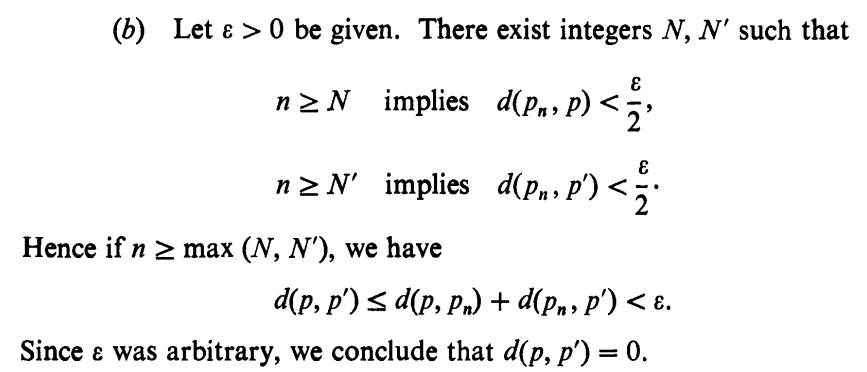
\includegraphics[width=0.9 \textwidth]{3_2b}}\\

\noindent As we can see, the two proofs are almost identical, with some minor additions in our formalization and a seperate lemma for the last statement. This is only possible due to the low complexity of the calculations involved. As we get to more elaborate proofs, these calculations will take a lot more space, so we have to further seperate from the original text.

\begin{forthel}
	\begin{definition}[BoundedBy]
		Let $a$ be a sequence. Let $K$ be a real number. $a$ is bounded by $K$ iff
		for every $n \ abs(a[n]) \leq K$.
	\end{definition}
	
	\begin{definition}[BoundedSequence]
		Let $a$ be a sequence. $a$ is bounded iff there exists a real number $K$ such that
		$a$ is bounded by $K$.
	\end{definition}
	
	\begin{signature}[MaxN]
		Let $a$ be a sequence. $maxN(a,N)$ is a real number such that
		(there exists $n$ such that $n \leq N$ and $maxN(a,N) = a[n]$) and
		(for every $n$ such that $n \leq N \ a[n] \leq maxN(a,N)$).
	\end{signature}
	
	\begin{theorem}[ConvergentImpBounded]
		Let $a$ be a sequence. Assume that $a$ converges. Then $a$ is bounded.
	\end{theorem}

	\begin{proof}
		Take a real number $x$ such that $a$ converges to $x$.
		Take $N$ such that for every $n$ such that $N < n \ dist(a[n],x) < 1$ (by Convergence, OnePos).
		Define $b[k] = abs(a[k])$ for $k$ in $\NN$.
		Take a real number $K$ such that \linebreak $K = max(1 + abs(x), maxN(b,N))$.
		
		\noindent Let us show that $a$ is bounded by $K$.
		\begin{subproof}
			Let us show that for every $n \ abs(a[n]) \leq K$.
			\begin{subproof} 
				Let $n$ be a natural number.
				We have $n \leq N$ or $n > N$.
				
				Case $n \leq N$.
				\begin{case}
					We have $abs(a[n]) = b[n] \leq maxN(b,N)$ (by MaxN).\\
					We have $maxN(b,N) \leq K$ (by MaxIneqDummy).\\
					Therefore $abs(a[n]) \leq K$ (by LeqTransitivity).
				\end{case}
				Case $n > N$.
				\begin{case}
					We have $dist(a[n],x) < 1$.\\
					We have $1 + abs(x) \leq K$ (by MaxIneq).
					
					$abs(a[n]) \dotequal abs(a[n] + 0)$ (by Zero)\\
					$\dotequal abs(a[n] + (x - x))$ (by Neg)\\
					$\dotequal abs(a[n] + ((-x) + x))$ (by ComAdd)\\
					$\dotequal abs((a[n] - x) + x)$ (by AssAdd).
					
					Hence $abs(a[n]) \leq abs(a[n] - x) + abs(x)$ (by AbsTriangleIneq).\\
					Hence $abs(a[n]) \leq dist(a[n],x) + abs(x)$.\\
					We have $dist(a[n],x) + abs(x) < 1 + abs(x)$ (by MixedAddInvariance).\\
					Hence $abs(a[n]) \leq 1 + abs(x)$ (by MixedTransitivity).\\
					Therefore $abs(a[n]) \leq K$ (by LeqTransitivity).
				\end{case}
			\end{subproof}
			Hence $a$ is bounded by $K$ (by BoundedBy).
		\end{subproof}
	\end{proof}
	
	\begin{definition}[LimitPointOfSet]
		Let $E$ be a set. Assume every element of $E$ is a real number. A limit point of $E$
		is a real number $x$ such that for every positive real number $\epsilon$ there exists an element
		$y$ of $E$ such that $y$ is an element of $Neighb(x,\epsilon)$ and $y \neq x$.
	\end{definition}
	
	\begin{theorem}[ConvLimitPoint]
		Let $E$ be a set. Assume every element of $E$ is a real number. Let $x$ be a limit point of $E$.
		Then there exists a sequence $a$ such that $a$ converges to $x$ and for every $n \ a[n]$ is an element of $E$.
	\end{theorem}

	\begin{proof}
		Let us show that for every $n$ such that $n > 0$ there exists an element $y$ of $E$ such that
		$y$ is an element of $Neighb(x,inv(n))$ and $y \neq x$.
		\begin{subproof}
			Assume $n > 0$.
			Then $inv(n)$ is a positive real number.\\
			Take an element $y$ of $E$ such that $y$ is an element of $Neighb(x,inv(n))$
			and $y \neq x$ (by LimitPointOfSet).
		\end{subproof}
	
		\noindent Define $a[n] =$ Case $n = 0 \rightarrow$ Choose an element $y$ of $E$ such that $y$ is an element of
		$Neighb(x,1)$ and $y \neq x$ in $y$,
		Case $n > 0 \rightarrow$ Choose an element $y$ of $E$ such that $y$ is an element of
		$Neighb(x,inv(n))$ and $y \neq x$ in $y$
		for $n$ in $\NN$.\\
		$a$ is a sequence.	
		Then for every $n \ a[n]$ is an element of $E$.
		
		\noindent Let us show that $a$ converges to $x$.
		\begin{subproof}
			Let $\epsilon$ be a positive real number.\\
			Take $N$ such that $1 < N \cdot \epsilon$ (by ArchimedeanAxiom, OnePos).
			
			\noindent Let us show that for every $n$ such that $N < n \ dist(a[n],x) < \epsilon$.
			\begin{subproof}
				Assume $N < n$. Then $n \neq 0$.
				Then $a[n]$ is an element of $E$ such that $a[n]$ is an element of $Neighb(x,inv(n))$.\\
				Hence $dist(a[n],x) < inv(n)$.
				
				\noindent Let us show that $inv(n) < \epsilon$.
				\begin{subproof}
					We have $N \cdot \epsilon < n \cdot \epsilon$ (by ComMult, MultInvariance).\\
					Hence $1 < n \cdot \epsilon$ (by 	TransitivityOfOrder).
					$inv(n)$ is positive.
					Hence $inv(n) \cdot 1 < inv(n) \cdot (n \cdot \epsilon)$ (by MultInvariance).\\
					We have $inv(n) \cdot 1 = inv(n)$ (by One).
					
					$inv(n) \cdot (n \cdot \epsilon) \dotequal 		(inv(n) \cdot n) \cdot \epsilon$ (by AssMult)\\
					$\dotequal 1 \cdot \epsilon$ (by InvDummy)\\
					$\dotequal \epsilon$ (by OneDummy).
				\end{subproof}
				Hence $dist(a[n],x) < \epsilon$ (by 		TransitivityOfOrder).
			\end{subproof}
		\end{subproof}
	\end{proof}
\end{forthel}

\noindent In LaTeX it is possible to overload the plus operator by adding a simple replacement command. On the other hand in ForTheL one has to use slightly different operators like ' $+'$ ' instead of ' $+$ ':

\begin{forthel}	
	\begin{definition}[SequenceSum]
	Let $a,b$ be sequences. \\$a \plusone b$ is a sequence such that for every $n \ (a \plusone b)[n] = a[n] + b[n]$.
	\end{definition}
	
	\begin{definition}[SequenceProd]
	Let $a,b$ be sequences. \\$a \cdotone b$ is a sequence such that for every $n \ (a \cdotone b)[n] = a[n] \cdot b[n]$.
	\end{definition}
	
	\begin{definition}[SequenceConstSum]
	Let $a$ be a sequence. Let $c$ be a real number. $c \plustwo a$ is a sequence such that for every $n \ (c \plustwo a)[n] = c + a[n]$.
	\end{definition}
	
	\begin{definition}[SequenceConstProd]
	Let $a$ be a sequence. Let $c$ be a real number. $c \cdottwo a$ is a sequence such that for every $n \ (c \cdottwo a)[n] = c \cdot a[n]$.
	\end{definition}

	\begin{definition}[SequenceDiv]
	Let $a$ be a sequence. Assume for every $n \ a[n] \neq 0$. $div(a)$ is a sequence such that for every $n \ (div(a))[n] = inv(a[n])$.
	\end{definition}
	
	\begin{theorem}[SumConv]
	Let $a,b$ be sequences. Let $x,y$ be real numbers. Assume $a$ converges to $x$ and $b$ converges to $y$.
	Then $a \plusone b$ converges to $x + y$.
	\end{theorem}
	\begin{proof}
	Let $\epsilon$ be a positive real number.
	Take a positive real number $\halfeps$ such that $\halfeps = inv(2) \cdot \epsilon$.
	Take $N1$ such that for every $n$ such that \linebreak $N1 < n \ dist(a[n],x) < \halfeps$ (by Convergence).
	Take $N2$ such that for every $n$ such that $N2 < n \ dist(b[n],y) < \halfeps$ (by Convergence).
	Take $N$ such that $N = max(N1,N2)$.
	Then $N1 \leq N$ and $N2 \leq N$.
	\\Let us show that for every $n$ such that $N < n \ dist((a \plusone b)[n],(x+y)) < \epsilon$.
	\begin{subproof}
	Assume $N < n$.
	\\We have $dist(a[n],x) < \halfeps$.
	We have $dist(b[n],y) < \halfeps$.
	\\$abs((a[n] + b[n]) - (x + y))$ 
	\\$\dotequal abs((a[n] + b[n]) + ((-x) + (-y)))$ (by MinusRule1)
	\\$\dotequal abs((-x) + ((a[n] + b[n]) - y))$ (by BubbleAdd)
	\\$\dotequal abs((-x) + (a[n] + (b[n] - y)))$ (by AssAdd)
	\\$\dotequal abs(((-x) + a[n]) + (b[n] - y))$ (by AssAdd)
	\\$\dotequal abs((a[n] - x) + (b[n] - y))$ (by ComAdd).
		\\
		
		We have $abs((a[n] - x) + (b[n] - y)) \leq abs(a[n] - x) + abs(b[n] - y)$  (by AbsTriangleIneq).
	\\Hence $abs((a[n] + b[n]) - (x + y)) \leq dist(a[n],x) + dist(b[n],y)$.
	\\Hence $dist(a[n],x) + dist(b[n],y) < \halfeps + \halfeps$ (by AddInvariance).
	\\Thus $abs((a[n] + b[n]) - (x + y)) < \halfeps + \halfeps$ (by MixedTransitivity).
	\\Therefore $dist((a \plusone b)[n],(x + y)) < \halfeps + \halfeps$.
	\\Hence the thesis (by TwoHalf).
	\end{subproof}
	\end{proof}
	
	\begin{lemma}[ConstConv]
	Let $c$ be a real number. Let $cn$ be a sequence such that for every $n \ cn[n] = c$.
	Then $cn$ converges to $c$.
	\end{lemma}
	\begin{proof}
	Let $\epsilon$ be a positive real number.
	\\Let us show that for every $n$ such that $0 < n \ dist(cn[n],c) < \epsilon$.
	\begin{subproof}
	Assume $0 < n$.
	$dist(cn[n],c) = dist(c,c) = 0$ (by IdOfInd).
	\\Hence $dist(cn[n],c) < \epsilon$.
	\end{subproof}
	\end{proof}
	
	\begin{theorem}[SumConstConv]
	Let $a$ be a sequence. \\Let $x,c$ be real numbers. Assume $a$ converges to $x$.
	\\Then $c \plustwo a$ converges to $c + x$.
	\end{theorem}
	\begin{proof}
	Define $cn[n] = c$ for $n$ in $\NN$.
	$cn$ is a sequence.
	\\Let us show that $c \plustwo a = (cn \plusone a)$.
	\begin{subproof}
	Let us show that for every $n \ (c \plustwo a)[n] = (cn \plusone a)[n]$.
	\begin{subproof}
	Let $n$ be a natural number.
	$$(c \plustwo a)[n] \dotequal c + a[n]
	\dotequal cn[n] + a[n]
	\dotequal (cn \plusone a)[n].$$
	\end{subproof}
	Hence $c \plustwo a = (cn \plusone a)$ (by SequenceEq).
	\end{subproof}
	$cn$ converges to $c$ (by ConstConv).
	\\Then $c \plustwo a$ converges to $c + x$ (by SumConv).
	\end{proof}
	
	\begin{theorem}[ProdConstConv]
	Let $a$ be a sequence. \\Let $x,c$ be real numbers. Assume $a$ converges to $x$.
	\\Then $c \cdottwo a$ converges to $c \cdot x$.
	\end{theorem}
	\begin{proof}
	Case $c = 0$.
	\begin{case}
	We have $c \cdot x = 0$.
	\\Let us show that for every $n \ (c \cdottwo a)[n] = 0$. 
	\begin{subproof}
	$$(c \cdottwo a)[n] \dotequal c \cdot a[n]
	\dotequal 0 \cdot a[n]
	\dotequal 0 \text{ (by ZeroMult)}.$$
	\end{subproof}
	Hence $c \cdottwo a$ converges to $c \cdot x$ (by ConstConv).
	\end{case}
	Case $c \neq 0$.
	\begin{case}
	Let $\epsilon$ be a positive real number. 
	\\(1)     Take a positive real number $\inveps$ such that $\inveps = inv(abs(c)) \cdot \epsilon$.
	\\Take $N$ such that for every $n$ such that $N < n \ dist(a[n],x) < \inveps$ (By Convergence).
	\\Let us show that for every $n$ such that $N < n \ dist(c \cdot a[n],c \cdot x) < \epsilon$.
	\begin{subproof}
	Assume $N < n$.
	\\$abs((c \cdot a[n]) - (c \cdot x)) \dotequal abs((c \cdot a[n]) +  ((-1) \cdot (c \cdot x))) (by MinusRule4)$ 
	\\$\dotequal abs((c \cdot a[n]) + (((-1) \cdot c) \cdot x))$ (by AssMult)
	\\$\dotequal abs((c \cdot a[n]) + ((c \cdot (-1)) \cdot x))$ (by ComMult)
	\\$\dotequal abs((c \cdot a[n]) + (c \cdot ((-1) \cdot x)))$ (by AssMult)
	\\$\dotequal abs((c \cdot a[n]) + (c \cdot (-x)))$ (by MinusRule4)
	\\$\dotequal abs(c \cdot (a[n] - x))$ (by Distrib)
	\\$\dotequal abs(c) \cdot abs(a[n] - x)$ (by AbsMult).
	\\$abs(c) \cdot dist(a[n],x) < abs(c) \cdot \inveps$ (by AbsPos, MultInvariance).
	\\Hence $abs((c \cdot a[n]) - (c \cdot x)) < abs(c) \cdot \inveps$.
	\\$abs(c) \cdot \inveps \dotequal abs(c) \cdot (inv(abs(c)) \cdot \epsilon)$ (by 1)
	\\$\dotequal (abs(c) \cdot inv(abs(c))) \cdot \epsilon$ (by AssMult)
	\\$\dotequal 1 \cdot \epsilon$ (by Inverse)
	\\$\dotequal \epsilon$ (by OneDummy).
	\\Therefore $dist(c \cdot a[n],c \cdot x) < \epsilon$.
	\end{subproof}
	\end{case}
	\end{proof}
	
\end{forthel}

\noindent The following lemma was developed for the purpose of working around repeating one subproof in the proof of the theorem 'ProdConv' twice. Surprisingly, the eprover takes a long time to apply this lemma, although the lemma itself is proved really quickly and every precondition is provided.

\begin{forthel}

	\begin{lemma}[ConstMultSum]
	Let $a,b$ be sequences. \\Let $x,y$ be real numbers such that for every $n\ b[n] = y \cdot (a[n] + (-x))$. \\Assume $a$ converges to $x$.
	Then $b$ converges to $0$.
	\end{lemma}
	\begin{proof}
	Define $sum[k] = (-x) + a[k]$ for $k$ in $\NN$.
	$sum$ is a sequence.
	\\Let us show that $sum$ converges to $0$.
	\begin{subproof}
	We have $sum = (-x) \plustwo a$.
	\\Hence $sum$ converges to $(-x) + x$ (by SumConstConv).
	\\$(-x) + x = 0$ (by ComAdd, Neg).
	\end{subproof}
	Let us show that for every $n\ b[n] = y \cdot sum[n]$.
	\begin{subproof}
	$b[n] \dotequal y \cdot (a[n] + (-x))$
	\\$\dotequal y \cdot ((-x) + a[n])$ (by ComAdd)
	\\$\dotequal y \cdot sum[n]$.
	\end{subproof}
	Hence $b = y \cdottwo sum$ (by SequenceEq).
	\\Therefore $b$ converges to $0$ (by ProdConstConv, ComMult, ZeroMult).
	\end{proof}
	
	\begin{theorem}[ProdConv]
	Let $a,b$ be sequences. Let $x,y$ be real numbers. Assume $a$ converges to $x$ and $b$ converges to $y$.
	\\Let $a \cdotone b$ be a sequence such that for every natural number $n \ (a \cdotone b)[n] = a[n] \cdot b[n]$.
	Then $a \cdotone b$ converges to $x \cdot y$.
	\end{theorem}
	\begin{proof}
	(1) Define $s1[k] = (a[k] - x) \cdot (b[k] - y)$ for $k$ in $\NN$.
	\\Let us show that $s1$ converges to $0$. 
	\begin{subproof}
    Assume $\epsilon$ is a positive real number. 
    Take a positive real number $\rooteps$ such that $\rooteps = sqrt(\epsilon)$ (by Sqrt).
    Take $N1$ such that for every $n$ such that $N1 < n \ dist(a[n],x) < \rooteps$ (by Convergence).
    Take $N2$ such that for every $n$ such that $N2 < n \ dist(b[n],y) < \rooteps$ (by Convergence).
    Take $N$ such that $N = max(N1,N2)$.
    \\Let us show that for every $n$ such that $N < n \ dist(s1[n],0) < \epsilon$.
    \begin{subproof}
    Assume $N < n$.
    \\$dist(a[n],x), dist(b[n],y)$ and $\rooteps$ are nonnegative.
    \\$dist(a[n],x) < \rooteps$ and $dist(b[n],y) < \rooteps$.
    \\$dist(a[n],x) \cdot dist(b[n],y) < \epsilon$ (by NonNegMultInvariance).
    \\Then $abs(a[n] - x) \cdot abs(b[n] - y) < \epsilon$ (by DistDefinition).
    \\Hence $abs(((a[n] - x) \cdot (b[n] - y)) - 0) < \epsilon$ (by AbsMult,  Zero, NegOfZero).
    \end{subproof}
	\end{subproof}
	(2) Define $s2[k] = (x \cdot (b[k] + (-y))) + (y \cdot (a[k] + (-x)))$ for $k$ in $\NN$.
	\\Let us show that $s2$ converges to $0$.
	\begin{subproof}
	(3) Define $s2a[k] = y \cdot (a[k] + (-x))$ for $k$ in $\NN$.
	\\(4) Define $s2b[k] = x \cdot (b[k] + (-y))$ for $k$ in $\NN$.
	$s2a, s2b$ are sequences.
	Define $sum1[k] = a[k] + (-x)$ for $k$ in $\NN$.
	\\Define $sum2[k] = b[k] + (-y)$ for $k$ in $\NN$.
	$sum1, sum2$ are sequences.
	\\$sum1 = (-x) \plustwo a$ and $sum2 = (-y) \plustwo b$ (by ComAdd, SequenceEq).
	\\$sum1, sum2$ converge to $0$ (by SumConstConv, Neg, ComAdd).
	\\We have $s2a = y \cdottwo sum1$ and $s2b = x \cdottwo sum2$ (by SequenceEq).
	\\$s2a, s2b$ converge to $0$ (by ConstMultSum). 
	\\Let us show that for every $n \ s2[n] = s2b[n] + s2a[n]$.
	\begin{subproof}
	$s2[n] \dotequal (x \cdot (b[n] + (-y))) + (y \cdot (a[n] + (-x)))$ (by 2)\\
	$\dotequal s2b[n] + s2a[n]$ (by 3, 4).
	\end{subproof}
	Hence $s2$ converges to $0$ (by SumConv).
	\end{subproof}
	(5) Define $s3[k] = (a[k] \cdot b[k]) - (x \cdot y)$ for $k$ in $\NN$.
	\\Let us show that $s3$ converges to $0$.
	\begin{subproof}
	Let us show that for every $n \ s3[n] = s1[n] + s2[n]$.
	\begin{subproof}
	$s3[n] \dotequal (a[n] \cdot b[n]) - (x \cdot y)$ (by 5)
	\\$\dotequal ((a[n] - x) \cdot (b[n] - y)) + ((x \cdot (b[n] - y)) + (y \cdot (a[n] - x)))$ (by Identity1)
	\\$\dotequal s1[n] + s2[n]$ (by 1, 2).
	\end{subproof}
	Hence $s3 = s1 \plusone s2$ (by SequenceEq).
	\\Therefore the thesis (by SumConv, Zero).
	\end{subproof}
	Let $\epsilon$ be a positive real number.
	Take $N$ such that for every $n$ such that $N < n \ dist(s3[n],0) < \epsilon$ (by Convergence).
	\\Let us show that for every $n$ such that $N < n \ dist(a[n] \cdot b[n],x \cdot y) < \epsilon$.
	\begin{subproof}
	Assume $N < n$.
	\\$dist(s3[n],0) \dotequal dist((a[n] \cdot b[n]) - (x \cdot y),0)$ (by 5)
	\\$\dotequal abs(((a[n] \cdot b[n]) - (x \cdot y)) - 0)$ (by DistDefinition)
	\\$\dotequal abs((a[n] \cdot b[n]) - (x \cdot y))$ (by NegOfZero, Zero)
	\\$\dotequal dist(a[n] \cdot b[n],x \cdot y)$ (by DistDefinition).
	\end{subproof}
	\end{proof}

\end{forthel}

\noindent The next theorem is a bit degenerate since the apparently "simple" equations used in Rudin took much more concretisation when trying to prove it with Alice. 
We simplified the proof as much as possible - the prover did not accept further simplifications.

\begin{forthel}
	
	\begin{theorem}[DivConv]
	Let $a$ be a sequence. Let $x$ be a real number \\such that $x \neq 0$. Assume $a$ converges to $x$. 
	Assume for every $n \ a[n] \neq 0$.
	Let $div(a)$ be a sequence such that for every natural number $n \\ (div(a))[n] = inv(a[n])$.
	Then $div(a)$ converges to $inv(x)$.
	\end{theorem}
	\begin{proof}
	Let $\epsilon$ be a positive real number.
	\\$abs(x) \neq 0$. 
	$2, inv(2), abs(x), abs(x) \cdot abs(x), -abs(x), ((-1) \cdot inv(2)) \cdot abs(x), (inv(2) \cdot abs(x)) + (-abs(x))$ are real numbers.
	\\We have $pos(2)$ and $pos(inv(2))$ and $pos(abs(x))$ and $pos(abs(inv(x)))$ and $pos(inv(2) \cdot \epsilon)$ and $pos(abs(x) \cdot abs(x))$ and $pos((inv(2) \cdot \epsilon) \cdot (abs(x) \cdot abs(x)))$ and
	$pos(inv(2) \cdot abs(x))$ and $pos(\epsilon \cdot (abs(x) \cdot abs(x)))$ and $pos(inv(2) \cdot abs(inv(x)))$ and $pos((\epsilon \cdot (abs(x) \cdot abs(x))) \cdot (inv(2) \cdot abs(inv(x))))$.
	\\Take a natural number $m$ such that for every $n$ such that \linebreak $m < n \  dist(a[n],x) < inv(2) \cdot abs(x)$ (by Convergence).
	\\Let us show that for every $n$ such that $m < n \ inv(2) \cdot abs(x) < abs(a[n])$.
	\begin{subproof}
	Assume $m < n$.
	\\$a[n], abs(a[n]), -abs(a[n]), abs(x) - abs(a[n]), x - a[n], abs(x - a[n]), a[n] - x, abs(a[n] - x), abs(x) + (-abs(a[n])), (abs(x) + (-abs(a[n]))) + (-abs(x))$ are real numbers.
	\\Let us show that $abs(x) - abs(a[n]) < inv(2) \cdot abs(x)$.
	\begin{subproof}
	$abs(x) - abs(a[n]) \leq abs(x - a[n])$ (by AbsTriangleIneq2).
	$abs(x - a[n]) = abs(-(x - a[n])) = abs(a[n] - x)$ (by AbsPosNeg, MinusRule1, MinusRule2, ComAdd).
	\\$abs(a[n] - x) < inv(2) \cdot abs(x)$ (by DistDefinition).
	Hence the thesis (by MixedTransitivity).
	\end{subproof}
	Let us show that $-abs(a[n]) < (-inv(2)) \cdot abs(x)$.
	\begin{subproof}
	$(abs(x) - abs(a[n])) + (-abs(x)) < (inv(2) \cdot abs(x)) + (-abs(x))$ (by MixedAddInvariance). 
	\\$(abs(x) - abs(a[n])) + (-abs(x)) = -abs(a[n])$ (by AssAdd, Neg, ComAdd, Zero).
	\\$-abs(a[n]) < (inv(2) \cdot abs(x)) + (-abs(x))$ (by AssAdd, Neg, Zero).
	\\\\$(inv(2) \cdot abs(x)) + (-abs(x)) \dotequal (inv(2) \cdot abs(x)) + ((-1) \cdot abs(x))$ (by MinusRule4)
	\\$\dotequal (inv(2) + (-1)) \cdot abs(x)$ (by DistribDummy)
	\\$\dotequal ((1 \cdot inv(2)) + (-(1 \cdot inv(1)))) \cdot abs(x)$ (by OneDummy, Inverse)
	\\$\dotequal ((1 \cdot inv(2)) + ((-1) \cdot inv(1))) \cdot abs(x)$ (by OneDummy, MinusRule4)
	\\$\dotequal ((1 \cdot inv(2)) + ((-1) \cdot inv(1))) \cdot abs(x)$ (by MinusRule4)
	\\$\dotequal (((1 \cdot 1) + (2 \cdot (-1))) \cdot inv(2 \cdot 1)) \cdot abs(x)$ (by InvAdd)
	\\$\dotequal ((1 + ((-1) \cdot 2)) \cdot inv(2)) \cdot abs(x)$ (by One, ComMult).
	\\\\$1 + ((-1) \cdot 2) \dotequal 1 + -(1 \cdot 2)$ (by MinusRule5)
	\\$\dotequal -(2 - 1)$ (by OneDummy, MinusRule3)
	\\$\dotequal -1$. 
	\end{subproof}
    Therefore $abs(a[n]) > -((-inv(2)) \cdot abs(x))$ (by OrdMirror, MinusRule2).
    \\$-((-inv(2)) \cdot abs(x)) = abs(x) \cdot inv(2)$ (by MinusRule5, MinusRule2, ComMult).
    \\Therefore $abs(a[n]) > abs(x) \cdot inv(2)$ (by TransitivityOfOrder).
	\end{subproof}
	Take $N1$ such that for every $n$ such that $N1 < n \ dist(a[n],x) < (inv(2) \cdot \epsilon) \cdot (abs(x) \cdot abs(x))$ (by Convergence). 
	Take $N2$ such that $N2 = max(N1,m)$.
	\\Let us show that for every $n$ such that $N2 < n \ dist(inv(a[n]),inv(x)) < \epsilon$.
	\begin{subproof}
	Assume $N2 < n$.
	Then we have $N1 < n$ and $m < n$.
	\\Let us show that $dist(inv(a[n]),inv(x)) < ((\epsilon \cdot (abs(x) \cdot abs(x))) \cdot (inv(2) \cdot abs(inv(x)))) \cdot (1 \cdot inv(abs(a[n])))$.
	\begin{subproof}
	$dist(inv(a[n]),inv(x)) \dotequal abs(inv(a[n]) - inv(x))$ (by DistDefinition)
	\\$\dotequal abs((1 \cdot inv(a[n])) - (1 \cdot inv(x)))$ (by OneDummy)
	\\$\dotequal abs((1 \cdot inv(a[n])) + ((-1) \cdot inv(x)))$ (by MinusRule5)
	\\$\dotequal abs(((1 \cdot x) + (a[n] \cdot (-1))) \cdot inv(a[n] \cdot x))$ (by InvAdd)
	\\$\dotequal abs((x + ((-1) \cdot a[n])) \cdot inv(a[n] \cdot x))$ (by OneDummy, ComMult)
	\\$\dotequal abs((x - a[n]) \cdot inv(a[n] \cdot x))$ (by MinusRule4)
	\\$\dotequal abs(x - a[n]) \cdot abs(inv(a[n]) \cdot inv(x))$ (by AbsMult, InvRule2)
	\\$\dotequal abs(inv(a[n]) \cdot inv(x)) \cdot abs(x - a[n])$ (by ComMult).
	\\We have $pos(abs(inv(a[n]) \cdot inv(x)))$ (by AbsPos, InvNotZero, NoZeroDivisors).
	\\$abs(x - a[n]) = dist(a[n],x)$ (by DistDefinition, DistSymm).
	\\$abs(inv(a[n]) \cdot inv(x)) \cdot abs(x - a[n]) < abs(inv(a[n]) \cdot inv(x)) \cdot ((inv(2) \cdot \epsilon) \cdot (abs(x) \cdot abs(x)))$ (by MultInvariance, DistDefinition).
	\\$abs(inv(a[n]) \cdot inv(x)) \cdot ((inv(2) \cdot \epsilon) \cdot (abs(x) \cdot abs(x))) \\ \dotequal (abs(inv(a[n])) \cdot abs(inv(x))) \cdot ((inv(2) \cdot \epsilon) \cdot (abs(x) \cdot abs(x)))$ (by AbsMult)
	\\$\dotequal ((inv(2) \cdot \epsilon) \cdot (abs(x) \cdot abs(x))) \cdot (abs(inv(a[n])) \cdot abs(inv(x)))$ (by ComMult)
	\\$\dotequal (inv(2) \cdot (\epsilon \cdot (abs(x) \cdot abs(x)))) \cdot (abs(inv(a[n])) \cdot abs(inv(x)))$ (by AssMult)
	\\$\dotequal ((\epsilon \cdot (abs(x) \cdot abs(x))) \cdot inv(2)) \cdot (abs(inv(a[n])) \cdot abs(inv(x)))$ (by ComMult) 
	\\$\dotequal (\epsilon \cdot (abs(x) \cdot abs(x))) \cdot (inv(2) \cdot (abs(inv(a[n])) \cdot abs(inv(x))))$ (by AssMult)
	\\$\dotequal (\epsilon \cdot (abs(x) \cdot abs(x))) \cdot (inv(2) \cdot (abs(inv(x)) \cdot abs(inv(a[n]))))$ (by ComMult)
	\\$\dotequal (\epsilon \cdot (abs(x) \cdot abs(x))) \cdot ((inv(2) \cdot abs(inv(x))) \cdot abs(inv(a[n])))$ (by AssMult)
	\\$\dotequal ((\epsilon \cdot (abs(x) \cdot abs(x))) \cdot (inv(2) \cdot abs(inv(x)))) \cdot abs(inv(a[n]))$ (by AssMult)
	\\$\dotequal ((\epsilon \cdot (abs(x) \cdot abs(x))) \cdot (inv(2) \cdot abs(inv(x)))) \cdot inv(abs(a[n]))$ (by AbsInv)
	\\$\dotequal ((\epsilon \cdot (abs(x) \cdot abs(x))) \cdot (inv(2) \cdot abs(inv(x)))) \cdot (1 \cdot inv(abs(a[n])))$ (by OneDummy).
	\end{subproof}
	$(\epsilon \cdot (abs(x) \cdot abs(x))) \cdot (inv(2) \cdot abs(inv(x))), 1 \cdot inv(abs(a[n])), 2 \cdot inv(abs(x)), dist(inv(a[n]), inv(x)),
	((\epsilon \cdot (abs(x) \cdot abs(x))) \cdot (inv(2) \cdot abs(inv(x)))) \cdot (1 \cdot inv(abs(a[n]))), ((\epsilon \cdot (abs(x) \cdot abs(x))) \cdot (inv(2) \cdot abs(inv(x)))) \cdot (2 \cdot inv(abs(x)))$ are real numbers.
	\\Let us show that \\$((\epsilon \cdot (abs(x) \cdot abs(x))) \cdot (inv(2) \cdot abs(inv(x)))) \cdot (1 \cdot inv(abs(a[n]))) < \epsilon$.
	\begin{subproof} 
	Let us show that $1 \cdot inv(abs(a[n])) < 2 \cdot inv(abs(x))$.
	\begin{subproof}
	We have $abs(a[n]) > abs(x) \cdot inv(2)$.
	\\Hence $abs(a[n]) \cdot inv(1) > abs(x) \cdot inv(2)$ (by InvOne, One).
	\\We have ($pos(abs(a[n]))$ and $pos(1)$) and ($pos(abs(x))$ and $pos(2)$).
	\\($abs(a[n]) \neq 0$ and $1 \neq 0$) and ($abs(x) \neq 0$ and $2 \neq 0$).
	\\Then $1 \cdot inv(abs(a[n])) < 2 \cdot inv(abs(x))$ (by InvSwapIneq).
	\end{subproof}
	$((\epsilon \cdot (abs(x) \cdot abs(x))) \cdot (inv(2) \cdot abs(inv(x)))) \cdot (1 \cdot inv(abs(a[n]))) \\< ((\epsilon \cdot (abs(x) \cdot abs(x))) \cdot (inv(2) \cdot abs(inv(x)))) \cdot (2 \cdot inv(abs(x)))$ (by MultInvariance).
	\\$((\epsilon \cdot (abs(x) \cdot abs(x))) \cdot (inv(2) \cdot abs(inv(x)))) \cdot (2 \cdot inv(abs(x))) \\\dotequal ((\epsilon \cdot (abs(x) \cdot abs(x))) \cdot (inv(abs(x)) \cdot inv(2))) \cdot (2 \cdot inv(abs(x)))$ (by ComMult, AbsInv)
	\\$\dotequal (((\epsilon \cdot (abs(x) \cdot abs(x))) \cdot inv(abs(x))) \cdot inv(2)) \cdot (2 \cdot inv(abs(x)))$ (by AssMult)
	\\$\dotequal ((\epsilon \cdot (abs(x) \cdot abs(x))) \cdot inv(abs(x))) \cdot (inv(2) \cdot (2 \cdot inv(abs(x))))$ (by AssMult)
	\\$\dotequal (\epsilon \cdot ((abs(x) \cdot abs(x)) \cdot inv(abs(x)))) \cdot ((inv(2) \cdot 2) \cdot inv(abs(x)))$ (by AssMult)
	\\$\dotequal (\epsilon \cdot ((abs(x) \cdot abs(x)) \cdot inv(abs(x)))) \cdot inv(abs(x))$ (by InvDummy, OneDummy)
	\\$\dotequal (\epsilon \cdot (abs(x) \cdot (abs(x) \cdot inv(abs(x))))) \cdot inv(abs(x))$ (by AssMult)
	\\$\dotequal (\epsilon \cdot abs(x)) \cdot inv(abs(x))$ (by Inverse, One)
	\\$\dotequal \epsilon \cdot (abs(x) \cdot inv(abs(x)))$ (by AssMult)
	\\$\dotequal \epsilon$ (by Inverse, One).
	\end{subproof}
	Hence the thesis (by TransitivityOfOrder).
	\end{subproof}
	\end{proof}
\end{forthel}

\noindent The next excerpt of Rudin's book shows how big the differences are in length. This is the most extreme case of additional concretisation we have to provide the prover.

\fbox{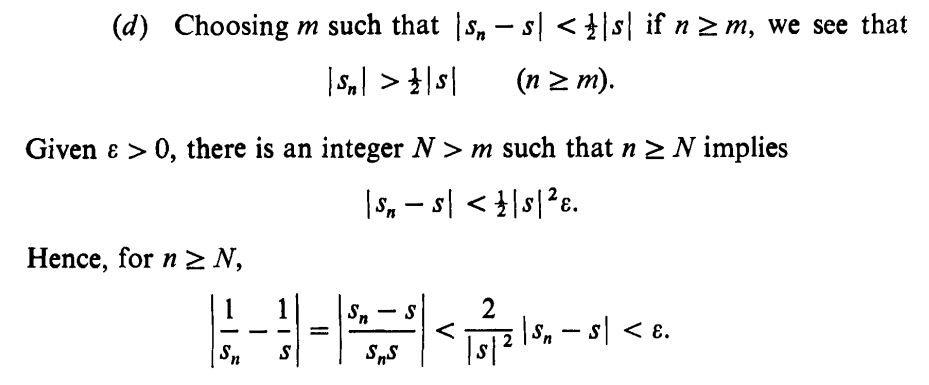
\includegraphics[width=0.9 \textwidth]{3_3d}}\\

\begin{forthel}	
	\begin{definition}[IndexSeq]
		An index sequence is a sequence $i$ such that \\
		(for every $n$ $i[n]$ is a natural number) and (for every $n$ $i[n] < i[n + 1]$).
	\end{definition}
	
	\begin{definition}[SubSeq]
		Let $a$ be a sequence and $i$ be an index sequence. $Subseq(a,i)$ is a sequence such that for every $n$
		$Subseq(a,i)[n] = a[i[n]]$.
	\end{definition}
	
	\begin{definition}[ConvSubSeq]
		Let $a$ be a sequence. $a$ has some convergent subsequence iff there exists an index sequence $i$ such that $Subseq(a,i)$ converges.
	\end{definition}
	
	\begin{axiom}[IndSucc]
		$n$ $\lessdot$ $n + 1$. 
	\end{axiom}
	
	\begin{axiom}[IndPrec]
		Assume $n \neq 0$. Then there exists $m$ such that \\ $n = m + 1$.
	\end{axiom}
	
	\begin{axiom}[IndNonNeg]
		$n \lessdot 0$ for no $n$.
	\end{axiom}
	
	\begin{axiom}[IndPlusOne]
		Assume $n < m$. Then $n + 1 \leq m$.
	\end{axiom}
	
	\begin{lemma}[SubSeqLeq]
		Let $a$ be a sequence. Let $i$ be an index sequence. Then for every $n$ $n \leq i[n]$.
	\end{lemma}
	
	\begin{proof}
		We can show by induction that $n \leq i[n]$ for every $n$.
		\begin{subproof}
			Let $n$ be a natural number.\\
			Case $n = 0$. Obvious.\\
			Case $n \neq 0$.
			\begin{case}
				Take $m$ such that $n = m + 1$. Then $m \leq i[m]$.\\
				We can show by induction that $i[k] + 1 \leq i[k + 1]$ for every $k$. Obvious.
			\end{case}
		\end{subproof}
	\end{proof}
	
	\begin{lemma}[LimitSubSeq]
		Let $a$ be a sequence. Let $x$ be a real number. \linebreak $a$ converges to $x$ iff for every index sequence $i$ $Subseq(a,i)$ converges to $x$. 
	\end{lemma}
	\begin{proof}
		Let us show that if $a$ converges to $x$ then for every index sequence $i$ $Subseq(a,i)$ converges to $x$.
		
		\begin{subproof}
			Assume $a$ converges to $x$. 
			Let $i$ be an index sequence.
			Let $\epsilon$ be a positive real number.
			Take $N$ such that for every $n$ such that $N < n$ $dist(a[n],x) < \epsilon$ (by Convergence).
			\\Let us show that for every $n$ such that $N < n$ \\ $dist(Subseq(a,i)[n],x) < \epsilon$.
			\begin{subproof}
				Let $n$ be a natural number such that $N < n$.\\
				Then $n \leq i[n]$ (by SubSeqLeq).\\
				Hence $N < i[n]$ (by MixedTransitivity).\\
				Hence $dist(Subseq(a,i)[n],x) = dist(a[i[n]],x) < \epsilon$.
			\end{subproof}
		\end{subproof}
		Let us show that if for every index sequence $i$ $Subseq(a,i)$ converges to $x$ then $a$ converges to $x$.
		\begin{subproof}
			Assume for every index sequence $i$ $Subseq(a,i)$ converges to $x$. \\
			Define $i[n] = n$ for $n$ in $\NN$.\\
			$i$ is an index sequence.\\
			$Subseq(a,i)$ converges to $x$. \\
			For every $n$ $a[n] = Subseq(a,i)[n]$. \\
			Hence $a = Subseq(a,i)$ (by SequenceEq). \\
			Hence $a$ converges to $x$.
		\end{subproof}
	\end{proof}
\end{forthel}

\noindent Rudin considers arbitrary metric spaces, so he shows that every convergent sequence is a cauchy sequence for all metric spaces and vice versa for $\RR^{n}$. We only consider the case of $\RR$, so we directly show the completeness of $\RR$. To achieve this we followed the proof found in \cite{Cauchy}.

\begin{forthel}
	\begin{axiom}[BolzanoWeierstrass]
		Let $a$ be a bounded sequence. Then $a$ has some convergent subsequence. 
	\end{axiom}
	
	\begin{definition}[Cauchy]
		A cauchy sequence is a sequence $a$ such that for every positive real number $\epsilon$ there exists $N$ such that
		for every $n$,$m$ such that ($N < n$ and $N < m$) $dist(a[n],a[m]) < \epsilon$.
	\end{definition}
	
	\begin{lemma}[CauchyBounded]
		Let $a$ be a cauchy sequence. Then $a$ is bounded.
	\end{lemma}
	\begin{proof}
		Take $N$ such that for every $n$,$m$ such that ($N < n$ and $N < m$) $dist(a[n],a[m]) < 1$ (by Cauchy, OnePos). \\
		$N + 1$ is a natural number and $N < N + 1$.\\
		Hence for every $n$ such that $N < n$ $dist(a[n],a[N + 1]) < 1$.\\
		Define $b[k] = abs(a[k])$ for $k$ in $\NN$.\\
		$maxN(b,N)$, $1$, $a[N + 1]$, $abs(a[N + 1])$, $1 + abs(a[N + 1])$ are real numbers.\\
		Take a real number $K$ such that $K = max(1 + abs(a[N + 1]), maxN(b,N))$.\\
		
		\noindent Let us show that $a$ is bounded by $K$.		
		\begin{subproof}
			Let us show that for every $n$ $abs(a[n]) \leq K$. 
			\begin{subproof}
				Let $n$ be a natural number.\\				
				$a[n]$, $abs(a[n])$, $b[n]$, $dist(a[n],a[N + 1])$, $a[n] - a[N + 1]$, $dist(a[n],a[N + 1]) + abs(a[N + 1])$ are real numbers.\\
				We have $n \leq N$ or $n > N$.\\
				Case $n \leq N$.
				\begin{case}
					We have $abs(a[n]) = b[n] \leq maxN(b,N)$ (by MaxN).
					
					We have $maxN(b,N) \leq K$ (by MaxIneqDummy).
					
					Therefore $abs(a[n]) \leq K$ (by LeqTransitivity).
					
				\end{case}	
				
				Case $n > N$.
				
				\begin{subproof}
					We have $dist(a[n],a[N + 1]) < 1$.\\
					We have $1 + abs(a[N + 1]) \leq K$ (by MaxIneq).\\
					
					$abs(a[n]) \dotequal abs(a[n] + 0)$ (by Zero)\\					
					$\dotequal abs(a[n] + (a[N + 1] - a[N + 1]))$ (by Neg)\\
					$\dotequal abs(a[n] + ((-a[N + 1]) + a[N + 1]))$ (by ComAdd)\\
					$\dotequal abs((a[n] - a[N + 1]) + a[N + 1])$ (by AssAdd).\\
					
					We have $abs((a[n] - a[N + 1]) + a[N + 1])\\ \leq abs(a[n] - a[N + 1]) + abs(a[N + 1])$ (by AbsTriangleIneq).\\
					Hence $abs(a[n]) \leq abs(a[n] - a[N + 1]) + abs(a[N + 1])$.\\
					Hence $abs(a[n]) \leq dist(a[n],a[N + 1]) + abs(a[N + 1])$.\\
					We have $dist(a[n],a[N + 1]) + abs(a[N + 1]) < 1 + abs(a[N + 1])$ (by MixedAddInvariance).\\
					Hence $abs(a[n]) \leq 1 + abs(a[N + 1])$ (by MixedTransitivity).\\
					Therefore $abs(a[n]) \leq K$ (by LeqTransitivity).
				\end{subproof}
			\end{subproof}
			Hence $a$ is bounded by $K$ (by BoundedBy).
		\end{subproof}
	\end{proof}
	
	\begin{lemma}[CauchyConvSubSeq]
		Let a be $a$ cauchy sequence such that $a$ has some convergent subsequence. Then $a$ converges.
	\end{lemma}
	
	\begin{proof}
		Take a index sequence $i$ such that $Subseq(a,i)$ converges.
		Take a real number $x$ such that $Subseq(a,i)$ converges to $x$.
		
		\noindent Let us show that $a$ converges to $x$.
		\begin{subproof}
			Let $\epsilon$ be a positive real number.\\			
			Take a positive real number $\halfeps$ such that $\halfeps = inv(2) \cdot \epsilon$.\\
			Take $N1$ such that for every $n$,$m$ such that ($N1 < n$ and $N1 < m$) $dist(a[n],a[m]) < \halfeps$ (by Cauchy).\\
			Take $N2$ such that for every $n$ such that $N2 < n$ $dist(Subseq(a,i)[n],x) < \halfeps$ (by Convergence).\\
			Take $N$ such that $N = max(N1,N2)$. Then $N1 \leq N$ and $N2 \leq N$.
			
			Let us show that for every $n$ such that $N < n$ $dist(a[n],x) < \epsilon$.
			\begin{subproof}
				Assume $N < n$. Hence $N1 < n$ and $N2 < n$ (by MixedTransitivity).\\
				We have $n \leq i[n]$ (by SubSeqLeq).\\
				Hence $N1 < i[n]$ (by MixedTransitivity).\\
				
				$a[n]$, $a[i[n]]$, $dist(a[n],a[i[n]])$, $dist(a[n],x), a[n] - a[i[n]], a[i[n]] - x$, $dist(a[n],a[i[n]]) + dist(a[i[n]],x)$ are real numbers.\\
				
				We have $Subseq(a,i)[n] = a[i[n]]$.\\
				We have $dist(a[n],a[i[n]]) < \halfeps$.\\
				We have $dist(a[i[n]],x) < \halfeps$.\\
				
				$dist(a[n],x) \dotequal abs(a[n] - x)$ (by DistDefinition)\\
				$\dotequal abs((a[n] + 0) - x)$ (by Zero)\\
				$\dotequal abs((a[n] + (a[i[n]] - a[i[n]])) - x)$ (by Neg)\\
				$\dotequal abs((a[n] + ((-a[i[n]]) + a[i[n]])) - x)$ (by ComAdd)\\
				$\dotequal abs(((a[n] - a[i[n]]) + a[i[n]]) - x)$ (by AssAdd)\\
				$\dotequal abs((a[n] - a[i[n]]) + (a[i[n]] - x))$ (by AssAdd).\\
				
				We have $abs((a[n] - a[i[n]]) + (a[i[n]] - x))\\ \leq abs(a[n] - a[i[n]]) + abs(a[i[n]] - x)$ (by AbsTriangleIneq).\\
				Hence $dist(a[n],x) \leq abs(a[n] - a[i[n]]) + abs(a[i[n]] - x)$.\\
				Hence $dist(a[n],x) \leq dist(a[n],a[i[n]]) + dist(a[i[n]],x)$.\\
				We have $dist(a[n],a[i[n]]) + dist(a[i[n]],x) < \halfeps + \halfeps$ (by AddInvariance).\\
				Hence $dist(a[n],x) < \halfeps + \halfeps$ (by MixedTransitivity).\\
				Hence $dist(a[n],x) < \epsilon$ (by TwoHalf).
			\end{subproof}
			
		\end{subproof}
	\end{proof}
	
	\begin{theorem}[RComplete]
		Let $a$ be a sequence. $a$ is a cauchy sequence iff $a$ converges.
	\end{theorem}
	
	\begin{proof}
		Let us show that (If $a$ converges then $a$ is a cauchy sequence).
		\begin{subproof}
			Assume $a$ converges.
			Take a real number $x$ such that $a$ converges \linebreak to $x$.
			Let $\epsilon$ be a positive real number.\\
			Take a positive real number $\halfeps$ such that $\halfeps = inv(2) \cdot \epsilon$.\\
			Take $N$ such that for every $n$ such that $N < n$ $dist(a[n],x) < \halfeps$ (by Convergence).
			
			Let us show that for every $n$,$m$ such that ($N < n$ and $N < m$) $dist(a[n],a[m]) < \epsilon$.
			\begin{subproof}
				Assume $N < n$ and $N < m$.\\
				We have $dist(a[n],x) < \halfeps$.\\
				We have $dist(a[m],x) < \halfeps$.\\
				We have $dist(a[n],a[m]) \leq dist(a[n],x) + dist(x,a[m])$ (by DistTriangleIneq).\\
				Hence $dist(a[n],a[m]) \leq dist(a[n],x) + dist(a[m],x)$ (by DistSymm).\\
				We have $dist(a[n],x) + dist(a[m],x) < \halfeps + \halfeps$ (by AddInvariance).\\
				Hence $dist(a[n],a[m]) < \halfeps + \halfeps$ (by MixedTransitivity).\\
				Hence $dist(a[n],a[m]) < \epsilon$ (by TwoHalf).
			\end{subproof}
		\end{subproof}
		
		\noindent Let us show that (If $a$ is a cauchy sequence then $a$ converges).
		\begin{subproof}
			Assume $a$ is a cauchy sequence.\\
			Then $a$ is bounded (by CauchyBounded).\\
			Therefore $a$ has some convergent subsequence (by BolzanoWeierstrass).\\
			Hence $a$ converges (by CauchyConvSubSeq).
		\end{subproof}
	\end{proof}
	
	
	\begin{definition}[MonInc]
		Let $a$ be a sequence. $a$ is monotonically increasing iff (for every $n$,$m$ such that $n \leq m$ $a[n] \leq a[m]$).
	\end{definition}
	
	\begin{definition}[MonDec]
		Let $a$ be a sequence. $a$ is monotonically decreasing iff (for every $n$,$m$ such that $n \leq m$ $a[n] \geq a[m]$).
	\end{definition}
	
	\begin{definition}[Mon]
		Let $a$ be a sequence. $a$ is monotonic iff $a$ is monotonically increasing or $a$ is monotonically decreasing.
	\end{definition}
	
	\begin{definition}[UpperBoundSeq]
		Let $a$ be a bounded sequence. Let $K$ be a real number. $K$ is upper bound of $a$ iff (for every $n$ $a[n] \leq K$).
	\end{definition}
	
	\begin{definition}[LeastUpperBoundSeq]
		Let $a$ be a bounded sequence. $LeastUpper(a)$ is a real number $K$ such that ($K$ is upper bound of $a$) and 
		(for every real number $L$ such that $L$ is upper bound of $a$ $K \leq L$).
	\end{definition}
	
	\begin{definition}[LowerBoundSeq]
		Let $a$ be a bounded sequence. Let $K$ be a real number. $K$ is lower bound of $a$ iff (for every $n$ $a[n] \geq K$).
	\end{definition}
	
	\begin{definition}[GreatestLowerBoundSeq]
		Let $a$ be a bounded sequence. $GreatestLower(a)$ is a real number $K$ such that ($K$ is lower bound of $a$) and
		(for every real number $L$ such that $L$ is lower bound of a $L \leq K$).
	\end{definition}
	
	\begin{lemma}[MonIncCon]
		Let $a$ be a monotonically increasing bounded sequence. Then $a$ converges.
	\end{lemma}
	
	\begin{proof}
		For every $n$ $a[n] \leq LeastUpper(a)$ (by UpperBoundSeq, LeastUpperBoundSeq).

		\noindent Let us show that for every positive real number $\epsilon$ there exists $N$ such that $(LeastUpper(a) - \epsilon) < a[N]$.
		\begin{subproof}
			Assume the contrary.\\
			Take a positive real number $\epsilon$ such that for every $N$ \linebreak$\neg$ ($(LeastUpper(a) - \epsilon) < a[N]$).
			
			Let us show that for every $n$ $a[n] \leq (LeastUpper(a) - \epsilon)$.
			\begin{subproof}
				Let $n$ be a natural number.\\
				We have $\neg$ ($(LeastUpper(a) - \epsilon) < a[n]$).\\
				Therefore $(LeastUpper(a) - \epsilon) \geq a[n]$ (by NotRuleOrder).\\
				Hence $a[n] \leq (LeastUpper(a) - \epsilon)$.
			\end{subproof}
			Hence $(LeastUpper(a) - \epsilon)$ is upper bound of $a$ (by UpperBoundSeq).
			
			$LeastUpper(a) - (LeastUpper(a) - \epsilon)\\ \dotequal LeastUpper(a) + (-LeastUpper(a) + \epsilon)$ (by MinusRule1, MinusRule2)\\
			$\dotequal (LeastUpper(a) - LeastUpper(a)) + \epsilon$ (by AssAdd)\\
			$\dotequal 0 + \epsilon$ (by Neg)\\
			$\dotequal \epsilon + 0$ (by ComAdd)\\
			$\dotequal \epsilon$ (by Zero).

			Hence $(LeastUpper(a) - \epsilon) < LeastUpper(a)$.\\
			Hence $\neg$ ($(LeastUpper(a) - \epsilon) \geq LeastUpper(a)) (by NotRuleOrder)$.\\
			Contradiction (by LeastUpperBoundSeq).
		\end{subproof}
		
		\noindent Let us show that $a$ converges to $LeastUpper(a)$.
		
		\begin{subproof}
			Let $\epsilon$ be a positive real number.\\
			Take $N$ such that $(LeastUpper(a) - \epsilon) < a[N]$.
			
			Let us show that for every $n$ such that $N < n$\\ $dist(a[n],LeastUpper(a)) < \epsilon$.
			\begin{subproof}
				Assume $N < n$.\\
				Hence $a[N] \leq a[n]$ (by MonInc).\\
				We have $a[n] \leq LeastUpper(a)$.\\
				Hence $dist(a[n],LeastUpper(a)) = abs(LeastUpper(a) - a[n])\\ = LeastUpper(a) - a[n]$.\\
				We have $(LeastUpper(a) - \epsilon) + \epsilon < a[N] + \epsilon$ (by MixedAddInvariance).\\
				We have $((LeastUpper(a) - \epsilon) + \epsilon) - a[N] < (a[N] + \epsilon) - a[N]$ (by MixedAddInvariance).\\
				
				$((LeastUpper(a) - \epsilon) + \epsilon) - a[N]\\
				\dotequal (LeastUpper(a) + (-\epsilon + \epsilon)) - a[N]$ (by AssAdd)\\
				$\dotequal (LeastUpper(a) + (\epsilon - \epsilon)) - a[N]$ (by ComAdd)\\
				$\dotequal (LeastUpper(a) + 0) - a[N]$ (by Neg)\\
				$\dotequal LeastUpper(a) - a[N]$ (by Zero).\\
				
				$(a[N] + \epsilon) - a[N]\\ \dotequal (\epsilon + a[N]) - a[N]$ (by ComAdd)\\
				$\dotequal \epsilon + (a[N] - a[N])$ (by AssAdd)\\
				$\dotequal \epsilon + 0$ (by Neg)\\
				$\dotequal \epsilon$ (by Zero).
				
				Hence $LeastUpper(a) - a[N] < \epsilon$.\\
				We have $LeastUpper(a) - a[n] \leq LeastUpper(a) - a[N]$.\\
				Hence $dist(a[n],LeastUpper(a)) < \epsilon$ (by MixedTransitivity).
			\end{subproof}
		\end{subproof}
	\end{proof}
\end{forthel}
	
\noindent Rudin writes that the other case of monotonically decreasing sequences works analogously, but obviously this is not possible in a strict proof system. Instead we decided to prove the other case by using that the negation of a monotonically decreasing sequence is monotonically increasing. Hence we can deduce the general case from the special case.
	
\begin{forthel}
	\begin{theorem}[MonCon]
		Let $a$ be a monotonic sequence. $a$ converges iff $a$ is bounded.
	\end{theorem}
	
	\begin{proof}
		We have (If $a$ converges then $a$ is bounded) (by ConvergentImpBounded).
		
		\noindent Assume $a$ is bounded.
		
		\noindent Case $a$ is monotonically increasing.
		\begin{case}
			Then $a$ converges (by MonIncCon). 
		\end{case} 
		Case $a$ is monotonically decreasing.
		\begin{subproof}
			Let us show that $(-1) \cdottwo a$ is monotonically increasing.
			
			\begin{subproof}
				Assume $n \leq m$.\\
				Then $a[n] \geq a[m]$ (by MonDec).\\
				Then $-a[n] \leq -a[m]$ (by OrdMirrorLeq).
				
				$((-1) \cdottwo a)[n] \dotequal (-1) \cdot a[n]
				\dotequal -a[n]$ (by MinusRule4).
				
				$((-1) \cdottwo a)[m] \dotequal (-1) \cdot a[m]
				\dotequal -a[m]$ (by MinusRule4).
				
				Hence $((-1) \cdottwo a)[n] \leq ((-1) \cdottwo a)[m]$.
			\end{subproof}
		
			Let us show that $(-1) \cdottwo a$ is bounded.
			\begin{subproof}
				Take a real number $K$ such that for every $n$ $abs(a[n]) \leq K$ (by BoundedSequence).
				
				Let us show that for every $n$ $abs(((-1) \cdottwo a)[n]) \leq K$.
				\begin{subproof}
					$abs(((-1) \cdottwo a)[n]) \dotequal abs((-1) \cdot a[n])$ (by SequenceConstProd)\\
					$\dotequal abs(-a[n])$ (by MinusRule4)\\
					$\dotequal abs(a[n])$ (by AbsPosNeg).
					
					Hence $abs(((-1) \cdottwo a)[n]) \leq K$.
				\end{subproof}
				Hence $(-1) \cdottwo a$ is bounded by $K$ (by BoundedBy).
			\end{subproof}
			Hence $(-1) \cdottwo a$ converges (by MonIncCon).\\
			Take a real number $x$ such that $(-1) \cdottwo a$ converges to $x$ (by Conv).
			
			Let us show that $(-1) \cdottwo ((-1) \cdottwo a) = a$.
			\begin{subproof}
				Let us show that for every $n$ $((-1) \cdottwo ((-1) \cdottwo a))[n] = a[n]$.
				\begin{subproof}
					Let $n$ be a natural number.
					
					$((-1) \cdottwo ((-1) \cdottwo a))[n] \dotequal (-1) \cdot ((-1) \cdottwo a)[n]$ (by SequenceConstProd)\\
					$\dotequal (-1) \cdot ((-1) \cdot a[n])$ (by SequenceConstProd)\\
					$\dotequal -(-a[n])$ (by MinusRule4)\\
					$\dotequal a[n]$ (by MinusRule2).
				\end{subproof}
				
				Hence $(-1) \cdottwo ((-1) \cdottwo a) = a$ (by SequenceEq).
			\end{subproof}
			
			Then $(-1) \cdottwo ((-1) \cdottwo a)$ converges to $(-1) \cdot x$ (by ProdConstConv).\\
			Hence $a$ converges (by Conv).
		\end{subproof}
	\end{proof}
	
	\noindent Let $b$ denote a real number. 
	\\Let $A, B, S$ denote a set.
	
	
	\begin{definition}[BoundedAboveBy]
		Let $S$ be a set. Assume every element of $S$ is a real number. Let $b$ be a real number. $S$ is bounded above by $b$ iff for every real number $x$ such that $x$ is an element of $S \ x \leq b$.
	\end{definition}
	
	\begin{definition}[BoundedAbove]
		Let $S$ be a set. Assume every element of $S$ is a real number. $S$ is bounded above iff there exists a real number $b$ such that $S$ is bounded above by $b$.
	\end{definition}
	
	\begin{definition}[BoundedBelowBy]
		Let $S$ be a set. Assume every element of $S$ is a real number. Let $b$ be a real number. $S$ is bounded below by $b$ iff for every real number $x$ such that $x$ is an element of $S \ x \geq b$.
	\end{definition}
	
	\begin{definition}[BoundedBelow]
		Let $S$ be a set. Assume every element of $S$ is a real number. $S$ is bounded below iff there exists a real number $b$ such that $S$ is bounded below by $b$.
	\end{definition}
	
	\begin{definition}[Sup] 
		Let $S$ be a set. Assume every element of $S$ is a real number. 
		Assume that $S$ is bounded above. Let $a$ be a real number such that $S$ is bounded above by $a$. 
		$sup(S) = a$ iff for every real number $b$ such that $b < a$ $S$ is not bounded above by $b$.
	\end{definition}
	
	\begin{definition}[Inf]
		Let $S$ be a set. Assume every element of $S$ is a real number. 
		Assume that $S$ is bounded below. Let $a$ be a real number such that $S$ is bounded below by $a$. 
		$inf(S) = a$ iff for every real number $b$ such that $b > a$ $S$ is not bounded below by $b$.
	\end{definition}
	
	\begin{definition}[LimSup]
		Let $a$ be a sequence. Let $E$ be a set such that \\$E = \{ x \mid x $ is a real number and there exists an index sequence i such that $ Subseq(a,i) \text{ converges to } x \}$. $limsup(a) = sup(E)$ iff $E$ is bounded above.
	\end{definition}
	
	\begin{definition}[LimInf]
		Let $a$ be a sequence. Let $E$ be a set such that $E = \{ x \mid x $ is a real number and there exists an index sequence i such that $ Subseq(a,i) \text{ converges to } x \}$. $limsup(a) = inf(E)$ iff $E$ is bounded below.
	\end{definition}
\end{forthel}

\subsection{helper.ftl}
In the following part we display basic propositions with rather technical proofs, which we needed to add as auxiliaries for the Rudin-Theorems.

\begin{forthel}
	\noindent [read Sequences/Naturals.ftl]\\
	Let $n,m$ denote natural numbers.\\
	Let $a,b,c,d$ denote real numbers.
	
	
	
	\begin{lemma}[MaxIneqDummy]
	Let $a,b$ be real numbers. $$b \leq max(a,b).$$
	\end{lemma}
	
	\begin{lemma}[NotRuleOrder]
	$a < b$ iff $\neg(a \geq b)$.
	\end{lemma}
	
	\begin{lemma}[MixedAddInvariance]
	$a < c \wedge b \leq d \Rightarrow a + b < c + d$.
	\end{lemma}
	
	\begin{lemma}[TwoHalf]
	$(inv(2) \cdot a) + (inv(2) \cdot a) = a$.
	\end{lemma}
	
\end{forthel}

\noindent In the following two lemmata we extended the minusrules from 'Reals.ftl'. Therefore the apparently strange enumeration.

\begin{forthel}
		
	\begin{lemma}[MinusRule5]
	Let $a,b$ be real numbers. 
	Then $$(a \cdot (-b)) = -(a \cdot b) \text{ and } ((-b) \cdot a) = -(b \cdot a).$$
	\end{lemma}
	\begin{proof} \\
	(1) $a \cdot (-b) \dotequal a \cdot ((-1) \cdot b)$ (by MinusRule4)
	\\$\dotequal (a \cdot (-1)) \cdot b$ (by AssMult)
	\\$\dotequal ((-1) \cdot a) \cdot b$ (by ComMult)
	\\$\dotequal (-1) \cdot (a \cdot b)$ (by AssMult)
	\\$\dotequal -(a \cdot b)$ (by MinusRule4).
	\\\\$((-b) \cdot a) \dotequal -(b \cdot a)$ (by ComMult, 1).
	\end{proof}
	
	\begin{lemma}[MinusRule6]
	Let $a,b$ be real numbers. 
	Then $$((-a) \cdot (-b)) = a \cdot b.$$
	\end{lemma}
	\begin{proof}\\
	$((-a) \cdot (-b)) \dotequal -(a \cdot (-b))$ (by MinusRule5)
	\\$\dotequal -(-(a \cdot b))$ (by MinusRule5)
	\\$\dotequal a \cdot b$ (by MinusRule2).
	\end{proof}
	
	\begin{lemma}[Binomi1]
	Let $a,b,c,d$ be real numbers.
	Then $$(a + b) \cdot (c + d) = ((a \cdot c) + (b \cdot c)) + ((a \cdot d) + (b \cdot d)).$$
	\end{lemma}
	\begin{proof}
	$(a + b) \cdot (c + d) \dotequal ((a + b) \cdot c) + ((a + b) \cdot d)$ (by Distrib)
	\\$\dotequal ((a \cdot c) + (b \cdot c)) + ((a \cdot d) + (b \cdot d))$ (by DistribDummy).
	\end{proof}
	
	\begin{lemma}[Binomi2]
	Let $a,b,c,d$ be real numbers.
	\\Then $(a - b) \cdot (c - d) = ((a \cdot c) - (b \cdot c)) + (-(a \cdot d) + (b \cdot d))$.
	\end{lemma}
	\begin{proof}
	$(a - b) \cdot (c - d) \dotequal ((a \cdot c) + ((-b) \cdot c)) + ((a \cdot (-d)) + ((-b) \cdot (-d)))$ (by Binomi1)
	\\$\dotequal ((a \cdot c) - (b \cdot c)) + (-(a \cdot d) + (b \cdot d))$ (by MinusRule5, MinusRule6).
	\end{proof}

	
\end{forthel}

\noindent The next identity is used in the theorem 'ProdConv', but in Rudin it was only mentioned without a proof. Since this is not an obvious result, we decided to prove it though. In the ForTheL-text we used the '.='-syntax in which one has to tell the eprover every rule he should use in each equation.
So this is a great example to visualize the amount of commands the eprover uses to transform simple algebraic equations (furthermore, the use of the rules Binomi2, MinusRule5 and MinusRule2 hides the use of plenty further rules).

\begin{forthel}
	
	\begin{lemma}[Identity1]
	Let $a,b,c,d$ be real numbers. 
	\\Then $(a \cdot b) - (c \cdot d) = ((a - c) \cdot (b - d)) + ((c \cdot (b - d)) + (d \cdot (a - c)))$.
	\end{lemma}
	\begin{proof}
	$((a - c) \cdot (b - d)) + ((c \cdot (b - d)) + (d \cdot (a - c))) 
	\dotequal (((a \cdot b) - (c \cdot b)) + (-(a \cdot d) + (c \cdot d))) + ((c \cdot (b - d)) + (d \cdot (a - c)))$ (by Binomi2)
	\\$\dotequal (((a \cdot b) - (c \cdot b)) + (-(a \cdot d) + (c \cdot d))) + (((c \cdot b) + (c \cdot (-d))) + ((d \cdot a) + (d \cdot (-c))))$ (by Distrib)
	\\$\dotequal (((a \cdot b) - (c \cdot b)) + (-(a \cdot d) + (c \cdot d))) + (((c \cdot b) + (-(c \cdot d))) + ((d \cdot a) + (-(d \cdot c))))$ (by MinusRule5)
	\\$\dotequal ((c \cdot b) + (-(c \cdot d))) + ((((a \cdot b) - (c \cdot b)) + (-(a \cdot d) + (c \cdot d))) + ((d \cdot a) + (-(d \cdot c))))$ (by BubbleAdd)
	\\$\dotequal ((c \cdot b) + (-(c \cdot d))) + (((a \cdot b) - (c \cdot b)) + ((-(a \cdot d) + (c \cdot d)) + ((a \cdot d) + (-(c \cdot d)))))$ (by AssAdd, ComMult)
	\\$\dotequal ((c \cdot b) + (-(c \cdot d))) + (((a \cdot b) - (c \cdot b)) + ((-(a \cdot d) + (c \cdot d)) + (-(-((a \cdot d) + (-(c \cdot d)))))))$ (by MinusRule2)
	\\$\dotequal ((c \cdot b) + (-(c \cdot d))) + (((a \cdot b) - (c \cdot b)) + ((-(a \cdot d) + (c \cdot d)) + (-(-(a \cdot d) + (c \cdot d)))))$ (by ComAdd, MinusRule3)
	\\$\dotequal ((c \cdot b) + (-(c \cdot d))) + (((a \cdot b) - (c \cdot b)) + 0)$ (by Neg)
	\\$\dotequal ((-(c \cdot d)) + (c \cdot b)) + (-(c \cdot b) + (a \cdot b))$ (by ComAdd, Zero)
	\\$\dotequal (-(c \cdot d)) + ((c \cdot b) + (-(c \cdot b) + (a \cdot b)))$ (by AssAdd)
	\\$\dotequal (-(c \cdot d)) + (((c \cdot b) -(c \cdot b)) + (a \cdot b))$ (by AssAdd)
	\\$\dotequal -(c \cdot d) + (0 + (a \cdot b))$ (by Neg)
	\\$\dotequal -(c \cdot d) + ((a \cdot b) + 0)$ (by ComAdd)
	\\$\dotequal -(c \cdot d) + (a \cdot b)$ (by Zero)
	\\$\dotequal (a \cdot b) - (c \cdot d)$ (by ComAdd).
	\end{proof}
	
	
	
	\begin{signature}[Sqrt]
	Let $x$ be a positive real number. \\$sqrt(x)$ is a positive real number such that $sqrt(x) \cdot sqrt(x) = x$.
	\end{signature}
	
	\begin{lemma}[AbsTriangleIneq2]
	Let $x,y$ be real numbers. Then $$abs(x) - abs(y) \leq abs(x - y).$$
	\end{lemma}
	\begin{proof}\\
	$abs(x) \dotequal abs(x + ((-y) + y))$ (by Zero, Neg, ComAdd)
	\\$\dotequal abs((x + (-y)) + y)$ (by AssAdd).
	\\$abs((x + (-y)) + y) \leq abs(x - y) + abs(y)$ (by AbsTriangleIneq).
	\\Hence $abs(x) \leq abs(x + (-y)) + abs(y)$.
	\\$abs(x) + (-abs(y)) \leq (abs(x - y) + abs(y)) + (-abs(y))$ (by LeqAddInvariance).
	\\$(abs(x - y) + abs(y)) + (-abs(y)) = abs(x - y)$ (by AssAdd, Neg, Zero).
	\\Hence $abs(x) - abs(y) \leq abs(x - y)$ (by LeqTransitivity).
	\end{proof}
	
	
	\begin{lemma}[InvAdd]
	Let $a,b,c,d$ be real numbers. \\Assume $(a \neq 0 \text{ and } b \neq 0) \text{ and } (c \neq 0 \text{ and } d \neq 0)$. 
	Then $$(a \cdot inv(b)) + (c \cdot inv(d)) = ((a \cdot d) + (b \cdot c)) \cdot inv(b \cdot d).$$
	\end{lemma}
	\begin{proof}\\
	$(a \cdot inv(b)) + (c \cdot inv(d)) \dotequal ((a \cdot inv(b)) \cdot 1) + (1 \cdot (c \cdot inv(d)))$ (by One, OneDummy)
	\\$\dotequal ((a \cdot inv(b)) \cdot (d \cdot inv(d))) + ((b \cdot inv(b)) \cdot (c \cdot inv(d)))$ (by Inverse)
	\\$\dotequal (a \cdot (inv(b) \cdot (d \cdot inv(d)))) + (b \cdot (inv(b) \cdot (c \cdot inv(d))))$ (by AssMult)
	\\$\dotequal (a \cdot ((inv(b) \cdot d) \cdot inv(d))) + (b \cdot ((inv(b) \cdot c) \cdot inv(d)))$ (by AssMult)
	\\$\dotequal (a \cdot ((d \cdot inv(b)) \cdot inv(d))) + (b \cdot ((c \cdot inv(b)) \cdot inv(d)))$ (by ComMult)
	\\$\dotequal (a \cdot (d \cdot (inv(b) \cdot inv(d)))) + (b \cdot (c \cdot (inv(b) \cdot inv(d))))$ (by AssMult)
	\\$\dotequal ((a \cdot d) \cdot (inv(b) \cdot inv(d))) + ((b \cdot c) \cdot (inv(b) \cdot inv(d)))$ (by AssMult)
	\\$\dotequal ((a \cdot d) \cdot inv(b \cdot d)) + ((b \cdot c) \cdot inv(b \cdot d)) $(by InvRule2)
	\\$\dotequal ((a \cdot d) + (b \cdot c)) \cdot inv(b \cdot d)$ (by DistribDummy).
	\end{proof}
	
	
	
	\begin{lemma}[InvCanc]
	Let $a, b$ be real numbers. Assume $a \neq 0$ and $b \neq 0$.
	Then $$(a \cdot inv(b)) \cdot (b \cdot inv(a)) = 1.$$
	\end{lemma}
	\begin{proof}
	$(a \cdot inv(b)) \cdot (b \cdot inv(a)) \dotequal ((a \cdot inv(b)) \cdot b) \cdot inv(a)$ (by AssMult)
	\\$\dotequal (a \cdot (inv(b) \cdot b)) \cdot inv(a)$ (by AssMult)
	\\$\dotequal (a \cdot 1) \cdot inv(a)$ (by InvDummy)
	\\$\dotequal a \cdot inv(a)$ (by One)
	\\$\dotequal 1$ (by Inverse).
	\end{proof}
	
	
	\begin{lemma}[NegMultInvariance]
	Let $x, y, z$ be real numbers.
	$$(x < y \wedge z < 0) \Rightarrow z \cdot x > z \cdot y.$$
	\end{lemma}
	\begin{proof}
	Assume $x < y \wedge z < 0$.
	Therefore $pos(-z)$.    
	Hence $(-z) \cdot x < (-z) \cdot y$.
	Hence $-((-z) \cdot x) > -((-z) \cdot y)$ (by OrdMirror).
	\\$-((-z) \cdot x) \dotequal (-(-z)) \cdot x$ (by MinusRule5)
	\\$\dotequal z \cdot x$ (by MinusRule2).
	\\$-((-z) \cdot y) \dotequal (-(-z)) \cdot y$ (by MinusRule5)
	\\$\dotequal z \cdot y$ (by MinusRule2).
	\end{proof}
	
	
	\begin{lemma}[InvSwapIneq]
	Let $a, b, c, d$ be positive real numbers. \\Assume $(a \neq 0$ and $b \neq 0)$ and $(c \neq 0 \text{ and } d \neq 0)$. 
	$$a \cdot inv(b) < c \cdot inv(d) \Rightarrow b \cdot inv(a) > d \cdot inv(c).$$
	\end{lemma}
	\begin{proof}
	Assume $a \cdot inv(b) < c \cdot inv(d)$.
	\\We have $pos(b \cdot inv(a))$ and $pos(d \cdot inv(c))$.
	\\$(b \cdot inv(a)) \cdot (a \cdot inv(b)) < (b \cdot inv(a)) \cdot (c \cdot inv(d))$ (by MultInvariance).
	\\$(b \cdot inv(a)) \cdot (a \cdot inv(b)) = $1 (by InvCanc).
	Hence $1 < (b \cdot inv(a)) \cdot (c \cdot inv(d))$.
	$(d \cdot inv(c)) \cdot 1 < (d \cdot inv(c)) \cdot ((b \cdot inv(a)) \cdot (c \cdot inv(d)))$ (by MultInvariance).
	$d \cdot inv(c) < (d \cdot inv(c)) \cdot ((b \cdot inv(a)) \cdot (c \cdot inv(d)))$ (by One).
	\\\\$(d \cdot inv(c)) \cdot ((b \cdot inv(a)) \cdot (c \cdot inv(d))) \\\dotequal ((b \cdot inv(a)) \cdot (c \cdot inv(d))) \cdot (d \cdot inv(c))$ (by ComMult)
	\\$\dotequal (b \cdot inv(a)) \cdot ((c \cdot inv(d)) \cdot (d \cdot inv(c)))$ (by AssMult)
	\\$\dotequal (b \cdot inv(a)) \cdot 1$ (by InvCanc)
	\\$\dotequal b \cdot inv(a)$ (by One).   
	\end{proof}
	
	
	
	\begin{lemma}[AbsInv]
	Let $x$ be a real number. Assume $x \neq 0$. Then $$abs(inv(x)) = inv(abs(x)).$$
	\end{lemma}
	\begin{proof} \\
	We have $pos(abs(inv(x)))$ and $pos(inv(abs(x)))$.
	$pos(1)$ (by OnePos).
	\\(1) Hence $( abs(inv(x)) = abs(abs(inv(x)))$ and $inv(abs(x)) = abs(inv(abs(x))) )$ and $abs(1) = 1$ (by AbsValue).
	\\$abs(inv(x)) \dotequal abs(abs(inv(x)))$ (by 1)
	\\$\dotequal abs(abs(inv(x)) \cdot 1)$ (by One)
	\\$\dotequal abs(abs(inv(x)) \cdot (abs(x) \cdot inv(abs(x))))$ (by Inverse)
	\\$\dotequal abs((abs(inv(x)) \cdot abs(x)) \cdot inv(abs(x)))$ (by AssMult)
	\\$\dotequal abs(abs(inv(x) \cdot x) \cdot inv(abs(x)))$ (by AbsMult)
	\\$\dotequal abs(abs(1) \cdot inv(abs(x)))$ (by InvDummy)
	\\$\dotequal abs(1 \cdot inv(abs(x)))$ (by 1) 
	\\$\dotequal abs(inv(abs(x)))$ (by OneDummy)
	\\$\dotequal inv(abs(x))$ (by 1).    
	\end{proof}
	
	
	\begin{lemma}[InvOne]
	$inv(1) = 1$.
	\end{lemma}
	\begin{proof}\\
	$1 \dotequal 1 \cdot inv(1)$ (by Inverse)
	\\$\dotequal inv(1)$ (by OneDummy).
	\end{proof}   
	
\end{forthel}


\section{Remarks}
\subsection{Structures}


\subsection{Text Comparisons}



\section{{From \LaTeX} to ForTheL}



\section{Discussion}


\begin{thebibliography}{1}

\bibitem{Rudin}
  Walter Rudin,
  \textit{Principles of mathematical analysis},
  McGraw-Hill,
  1976.
  
\bibitem{Cauchy}
	Mathe f\"ur Nicht-Freaks,
	\textit{Cauchy-Folgen und das Cauchy-Kriterium},
	\url{https://de.wikibooks.org/wiki/Mathe_f%C3%BCr_Nicht-Freaks:_Cauchy-Folgen_und_das_Cauchy-Kriterium},
	2018.

\end{thebibliography}
  


\end{document}
